\documentclass[tikz,border=10pt]{standalone}
\usetikzlibrary{arrows,intersections}
\begin{document}
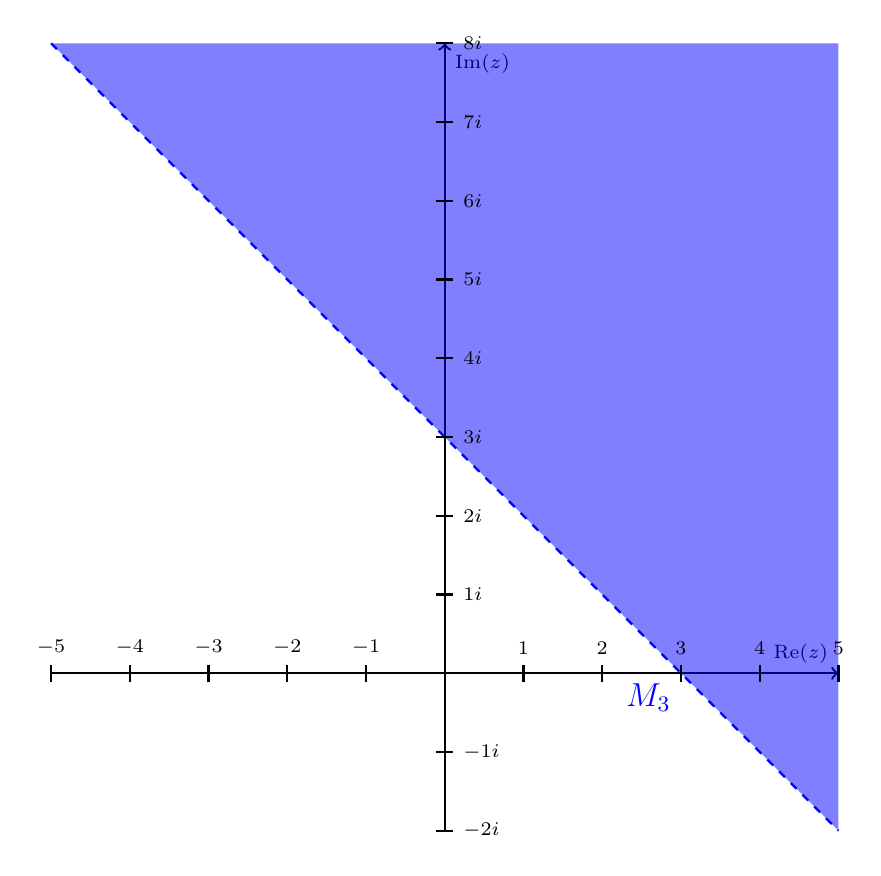
\begin{tikzpicture}
    \begin{scope}[thick,font=\scriptsize]

        \draw [->] (-5,0) -- (5,0) node [above left]  {Re$(z)$};
        \draw [->] (0,-2) -- (0,8) node [below right] {Im$(z)$};

        \draw [color=blue, dashed](-5,8)--(5,-2) node[pos=0.8, below left] {\large$M_3$};
        \path [draw=none,fill=blue,opacity = 0.5] (5,8) -- (-5,8) -- (5,-2);


        \foreach \n in {-2,...,-2,-1,1,2,...,5}{%
            \draw (\n,-3pt) -- (\n,3pt)   node [above] {$\n$};
            \draw (-3pt,\n) -- (3pt,\n)   node [right] {$\n i$};
        }
            \draw (-3,-3pt) -- (-3,3pt)   node [above] {$-3$};
            \draw (-4,-3pt) -- (-4,3pt)   node [above] {$-4$};
            \draw (-5,-3pt) -- (-5,3pt)   node [above] {$-5$};
            \draw (-3pt,6) -- (3pt,6)   node [right] {$6 i$};
            \draw (-3pt,7) -- (3pt,7)   node [right] {$7 i$};
            \draw (-3pt,8) -- (3pt,8)   node [right] {$8 i$};
    \end{scope}

\end{tikzpicture}
\end{document}
